\chapter{Finanzierung}
\section{Zentrale Annahmen}
\begin{itemize}
	\item Förderungen/Zuschüsse sind in den Berechnungen für den Kapitalbedarf nicht enthalten. Diese werden \ggf für den Kapitalbedarfsausgleich verwendet.
	\item Keine Gewinnausschüttung bzw. Bonifikationen an die Unternehmensgründer
	\item Zahlungsziele (Kunden und Lieferanten): 30 Tage
\end{itemize}

\section{Finanzierungsmodell}
Die laufende Finanzierung des Geschäftsmodells erfolgt durch 3 Säulen. 

\noindent
\begin{tabular}{@{}>{\raggedright\arraybackslash}p{1.8cm}@{}>{\raggedright\arraybackslash}p{\textwidth - 1.8cm}}
 
	Säule 1: & \textbf{Entwicklungskosten:}\\
	& Ein Hersteller oder ein Betreiber finanziert die Anpassung des System an einen speziellen Roboter mit der Entwicklungsgebühr. Die Anpassung an eine neue Version des Grundsystems kann ebenfalls in Auftrag gegeben werden.\\ 

	Säule 2: & \textbf{Lizenzgebühren}\\
	& Die Verwendung des Systems ist lizenziert. Für jeden Roboter, in dem das System zum Einsatz kommt, ist eine jährliche Lizenzgebühr fällig. Diese ist von verschiedenen Faktoren abhängig. \\
	
	Säule 3: & \textbf{Schulungskosten:}\\
	& Damit der Betreiber das System verwenden kann, müssen seine Mitarbeiter kostenpflichtig bei uns geschult werden. Dazu gibt es zwei unterschiedliche Varianten, die Grundschulung und die Expertenschulung.
\end{tabular}

\subsection{Entwicklungskosten}
\subsubsection{Neuentwicklung}
Die Entwicklungsgebühr ist unabhängig vom Roboter und Hersteller. Sie stützt sich darauf, dass der Roboter für die Betreiber attraktiver wird, da dieser eine jährliche Stromersparnis und dadurch resultierende Kostenersparnis mit sich bringt.\\
Die Entwicklungsgebühr beträgt $100.000,00$ \officialeuro.\\
Diese kann um bis zu $20$\% verringert werden sofern entsprechende Gegenleistungen angeboten werden.\\
Das Recht zur Vermarktung des angepassten Systems verbleibt jedoch ausnahmslos bei \textsf{RTI GmbH}.

\subsubsection{Weiterentwicklung}
Das grundlegende System unterliegt einer ständigen Weiterentwicklung. Neue Versionen des Systems müssen jedoch wieder an einen Roboter angepasst werden. Abhängig von den Versionsunterschieden und deren Aufwand zur Anpassung beträgt die Gebühr zwischen $25.000$ und $50.000$ \officialeuro.\\
Diese kann um bis zu $20$\% verringert werden sofern entsprechende Gegenleistungen angeboten werden.

\subsection{Lizenzgebühren}
Die Verwendung des Systems verschafft dem Betreiber einen enormen Wettbewerbsvorteil. Damit der Betreiber das System verwenden kann ist zurzeit eine einmalige Lizenzgebühr pro Roboter fällig. Sie wird wie folgt berechnet:\\
\begin{align*}
	\text{Gebühr} = [\{(24h * 365d * \varnothing A)*P_N\}*\varnothing K_{Strom}*E_N]*\frac{\varnothing B_N}{2} + IBN
\end{align*}
\begin{tabbing}
	\hspace{1,8cm}\=\hspace{0,6cm}\=\kill
	$\varnothing A$ \> \dots \> durchschnittliche Auslastung des Roboters in einem Jahr $[\%]$\\ 
	$P_N$\> \dots \> nominelle Leistungsaufnahme des Roboters bei deaktiviertem System\\ 
	\> \> (wird durch den eigenen Messaufbau festgelegt)\\
	$\varnothing K_{Strom}$\> \dots \> durchschnittliche gewerbliche Stromkosten\\ 
	$E_N$\> \dots \> Effizientssteigerung durch das System\\ 
	\> \> (wird durch den eigenen Messaufbau festgelegt) \\
	$\varnothing B_N$ \> \dots \> durchschnittliche nominelle Betriebsdauer des Roboters \\
	$IBN$ \> \dots \> Pauschale zur Inbetriebnahme
\end{tabbing}
Die Werte $P_N$ und $E_N$ sind abhängig von der Version des Systems und müssen für jede Version immer neu ermittelt werden. Die durchschnittliche Betriebsdauer $\varnothing B_N$ wird mit $10$ Jahren festgelegt und die durchschnittliche Auslastung $\varnothing A$ mit $70$\%. Ausnahmen können mit dem Betreiber explizit verhandelt werden. Die $IBN$-Pauschale ist ein fixer Wert und mit $350$ \officialeuro~ festgelegt. Für die durchschnittlichen Stromkosten wird der offizielle Wert der \textsf{E-CONTROL}\footnote{Energie-Control Austria für die Regulierung der Elektrizitäts- und Erdgaswirtschaft, Rudolfsplatz 13a, 1010 Wien} für Nicht-Haushalte über $150.000$MWh/Jahr Stromverbrauch herangezogen. Für die Berechnung gilt immer der zuletzt veröffentlichte Wert.\\
Für die \textit{Version 1} des Systems ergeben sich somit die Werte in Tabelle \ref{tab:Kalkulationswerte}.
\begin{table}[h]
	\centering
	\begin{tabular}{|c|c|}
		\hline 
		$\varnothing A$ & $70$\% \\ 
		\hline 
		$\varnothing K_{Strom}$ & $5,418\frac{\text{Cent}}{\text{kWh}}$ \\ 
		\hline
		$\varnothing B_N$ & $10$ Jahre \\ 
		\hline 
		$IBN$ & $350$\officialeuro \\ 
		\hline 
	\end{tabular}
	\caption{Kalkulationswerte für \textit{Version 1}}
	\label{tab:Kalkulationswerte}
\end{table}
Abschließend wird die Gebühr noch auf die Hunderter-Stelle gerundet. Die Gebühr bewegt sich somit in einem Bereich von $400,00$ \officialeuro~ -- $8.700,00$ \officialeuro~ für $E_N = 5,00$\% -- $50,00$\% und $P_N = 0,5$ kW -- $10,0$ kW. Eine grafische Verteilung der Lizenzgebühr ist in Abbildung \ref{fig:lizenzgebuehr} dargestellt.

\begin{figure}[h]
	\centering
	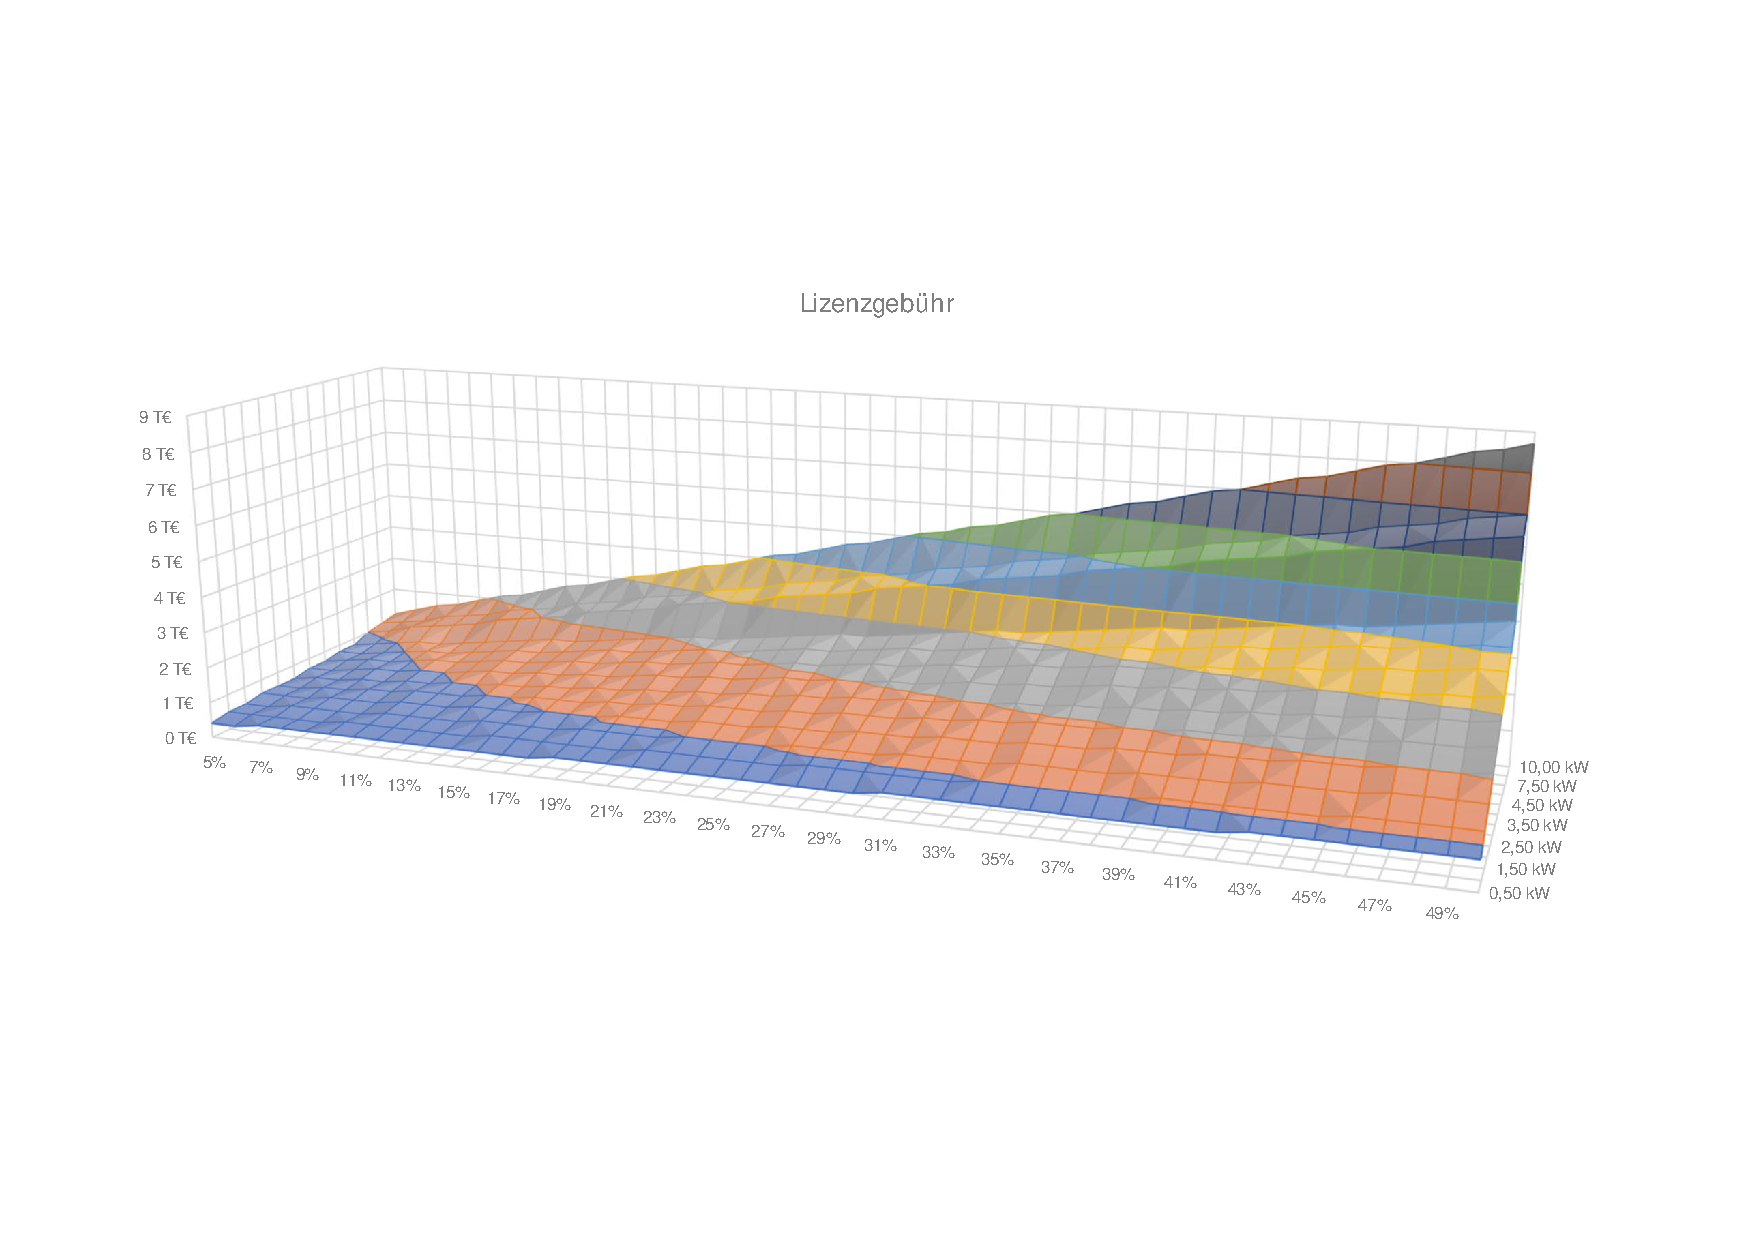
\includegraphics[width=15cm]{Lizenzgebuehr.pdf}
	\caption{Lizenzgebühr für die \textit{Version 1}}
	\label{fig:lizenzgebuehr}
\end{figure}

\paragraph*{Versionsupdate:}
Wird eine neue Version veröffentlicht, ist es für jeden Betreiber möglich auf das neue System upzudaten. Damit wird aber auch die Lizenzgebühr entsprechend angepasst. Außerdem wird die entsprechende $IBN$-Pauschale verrechnet.

\subsection{Schulungskosten}
\subsubsection{Grundschulung}
Die Grundschulung richtet sich an die Betreiber (Inbetriebnahme) und die Hersteller (Testcenter, Schulungscenter). Sie umfasst die Installation und Verwendung des System mit der Robotersteuerung. Die Schulung dauert zwei Tage und die Kosten betragen $800,00$ \officialeuro~ pro Person. 

\subsubsection{Expertenschulung}
Diese Schulung richtet sich grundsätzlich nur an die Betreiber (Inbetriebnahme). Im System können Parameter verändert werden um mögliche spezielle Anforderungen abdecken zu können. Wie die Parameter verändert werden können und welche Auswirkung die Veränderungen haben ist Teil der Expertenschulung. Diese dauert drei Tage und die Kosten betragen $1.500,00$ \officialeuro~ pro Person.

\section{Basis-Szenario}
Für das Basis-Szenario wurden folgende Annahmen getroffen:
\begin{itemize}
	\item Es werden in den folgenden vier Jahren 20 Neuentwicklungen in Auftrag gegeben (Aufteilung:~3/5/6/6). Damit werden $~12$\% der Robotertypen der fünf wichtigsten Hersteller mit dem System ausgerüstet, siehe Kapitel \ref{sec:Marketing}.
	\item Die Lizenzvergabe verteilt sich wie folgt:\newline (Angaben in Prozent vom weltweitem Absatz von Industrierobotern ($400.000$ Stück), siehe Kapitel \ref{sec:Marketing})
	\begin{itemize}
		\item 1. Jahr: 0 Roboter
		\item 2. Jahr: 120 Roboter
		\item 3. Jahr: 360 Roboter
		\item 4. Jahr: 1000 Roboter
	\end{itemize}
	\item Die durchschnittliche Lizenzgebühr beträgt $1.500,00$ \officialeuro.\\ Dies entspricht dem Mittelwert für $P_N = 1,50$ kW -- $5,00$ kW und $E_N = 10$\% -- $30$\%.
	\item Es wird mit 60 Teilnehmer an der Grundschulung innerhalb der nächsten vier Jahren gerechnet (Aufteilung:~8/12/16/24). Zusätzlich nehmen zehn Teilnehmer die Expertenschulung in Anspruch (Aufteilung: 0/2/3/5).
\end{itemize}

\newpage
\subsection{Break-Even-Point}
\label{sec:BasisSzenario-BEP}
Der BEP wird im Basis-Szenario knapp im zweiten Jahr erreicht, siehe Abbildung \ref{fig:BasisSzenario-BEP}.
\begin{figure}[h]
	\centering
	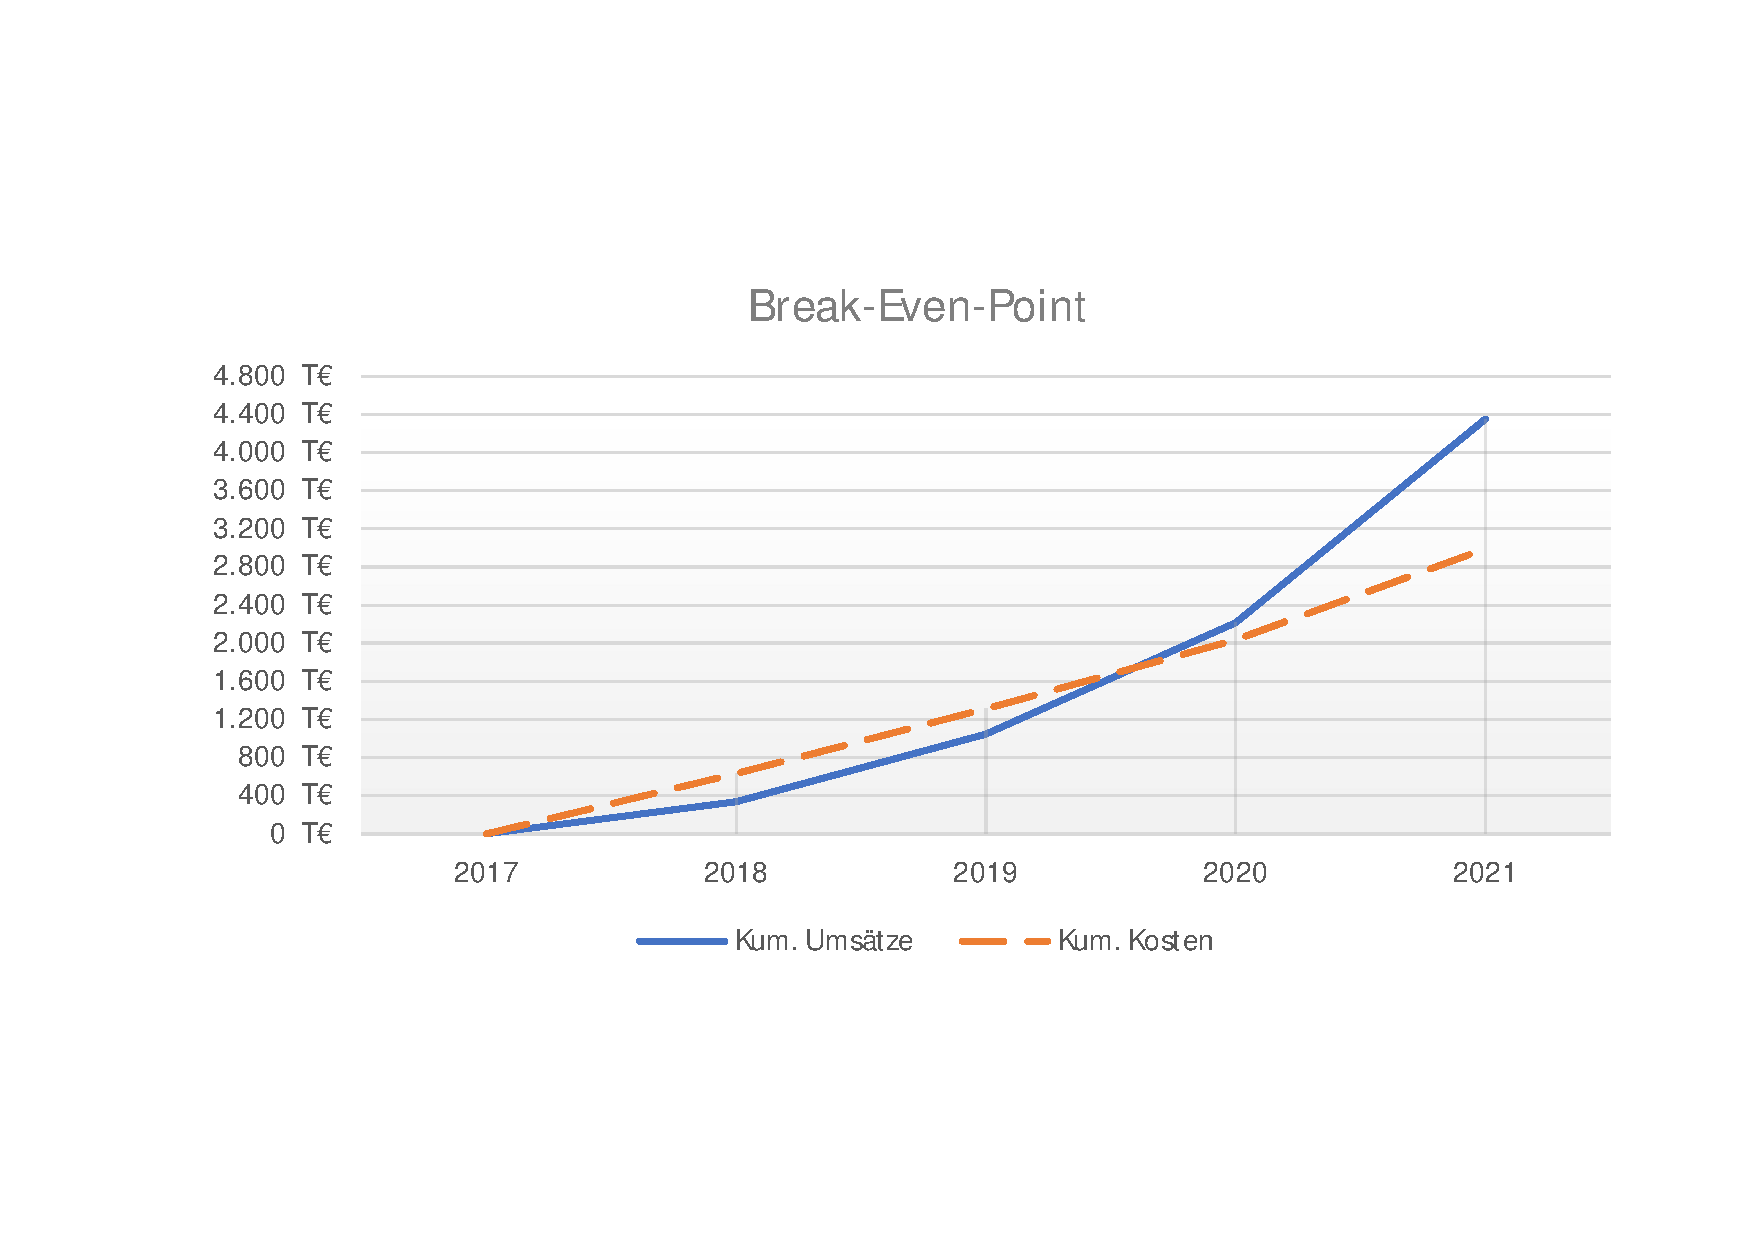
\includegraphics[width=15cm]{BasisSzenario-BEP.pdf}
	\caption{Break-Even-Point im Basis-Szenario}
	\label{fig:BasisSzenario-BEP}
\end{figure}\\
\\Die Netto-Umsätze und Kosten (pro Jahr und kumuliert) der nächsten vier Jahre sind in Tabelle \ref{tab:BasisSzenario-BEP} dargestellt.
\begin{table}[h]
	\centering
	\begin{tabular}{|l|c|c|c|c|}
		\hline 
		& 1. Jahr & 2. Jahr & 3. Jahr & 4. Jahr \\ 
		\hline 
		Umsätze & $338.953,63$ \officialeuro & $712.984,67$ \officialeuro & $1.175.701,33$ \officialeuro & $2.142.555,54$ \officialeuro \\
		\hline 
		Kosten & $545.926,40$ \officialeuro & $531.513,47$ \officialeuro & $624.473,73$ \officialeuro & $876.439,67$ \officialeuro \\		
		\hline 
		kum. Umsätze & $338.953,63$ \officialeuro & $1.051.938,30$ \officialeuro & $2.227.639,63$ \officialeuro & $4.370.195,17$ \officialeuro \\		
		\hline 
		kum. Kosten & $545.926,40$ \officialeuro & $1.077.439,87$ \officialeuro & $1.701.913,60$ \officialeuro & $2.578.353,27$ \officialeuro \\		
		\hline 
	\end{tabular}
	\caption{Umsätze und Kosten des Basis-Szenarios}
	\label{tab:BasisSzenario-BEP} 
\end{table}\\
Dadurch ergibt sich eine maximale Differenz der kumulierten Werte von $206.972,76$ \officialeuro.

\newpage
\subsection{Kennzahlen}
\begin{figure}[h]
	\centering
	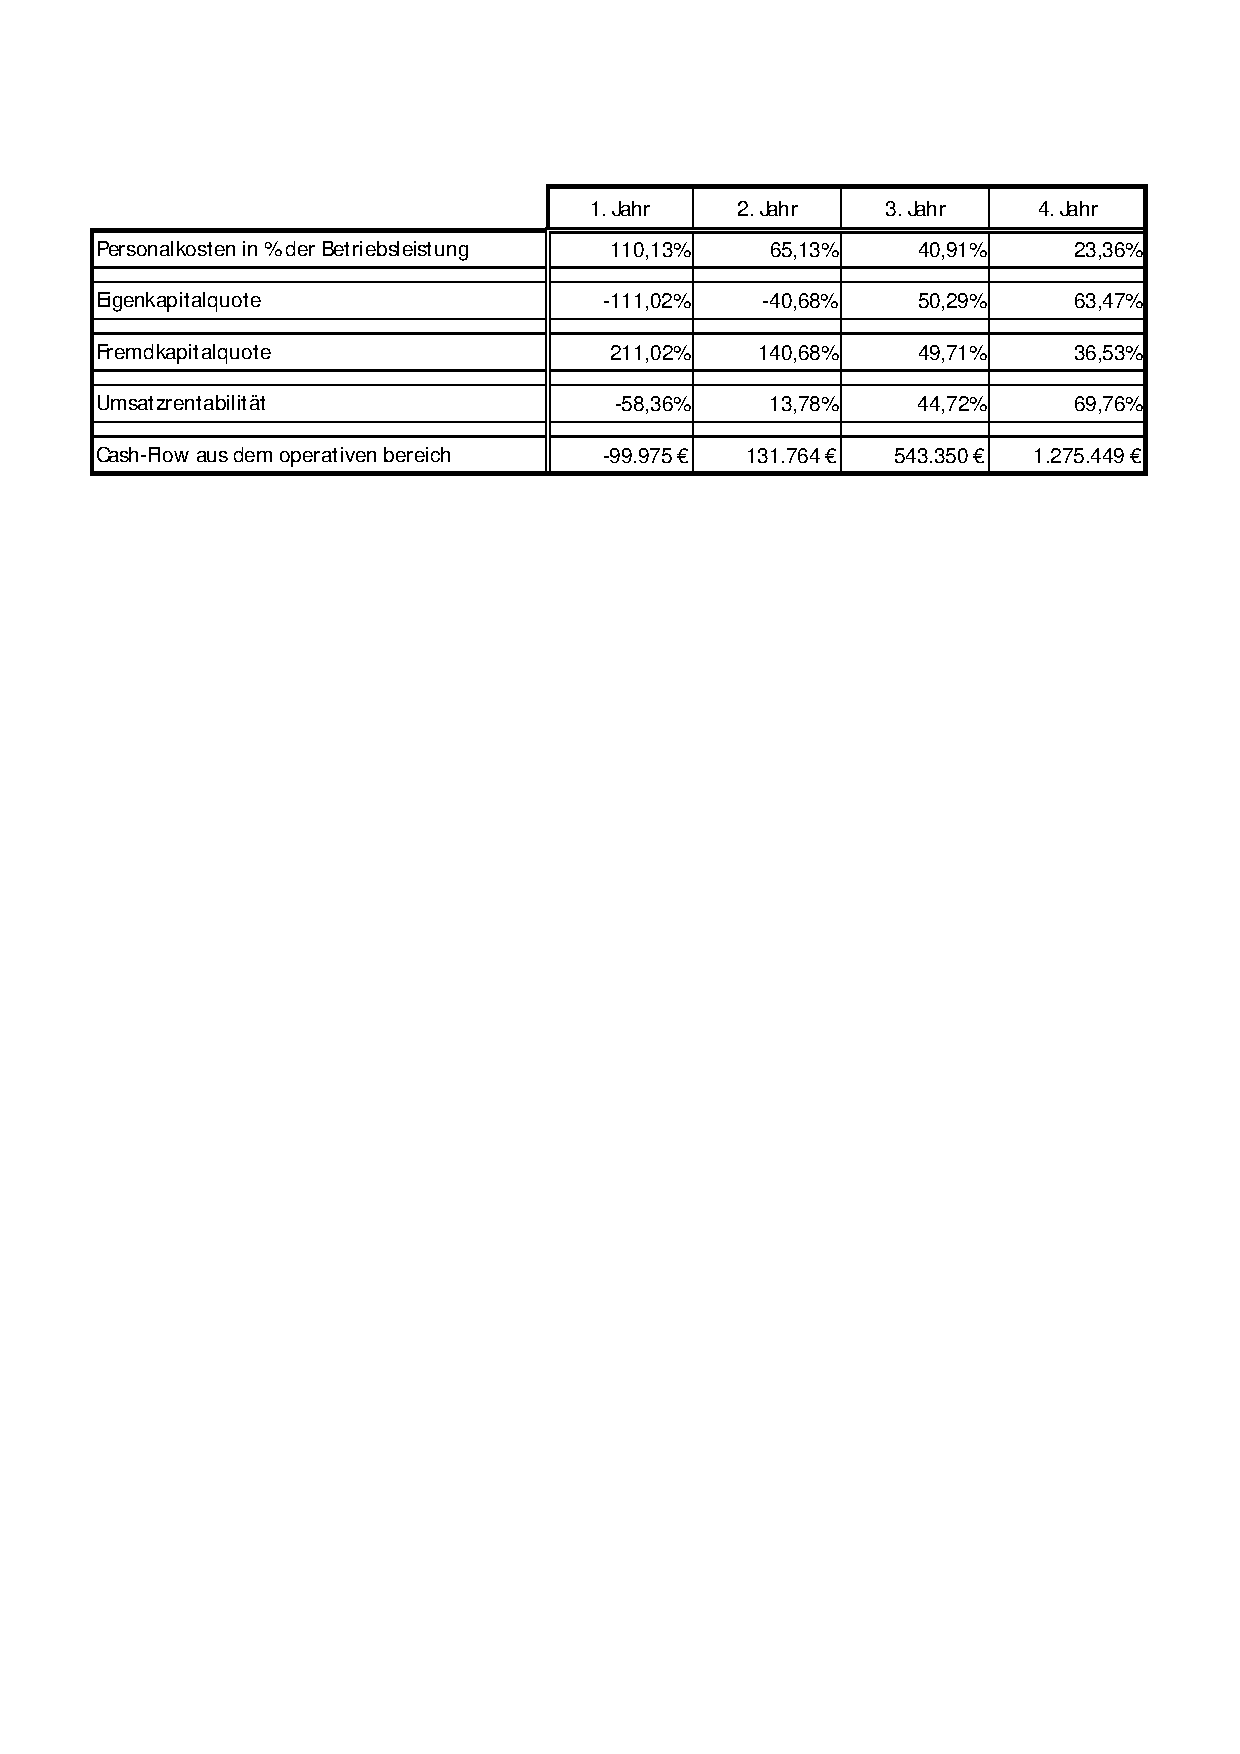
\includegraphics[width=15cm]{BasisSzenario-Kennzahlen.pdf}
	\caption{Kennzahlen im Basis-Szenario}
	\label{fig:BasisSzenario-Kennzahlen}
\end{figure}
\newpage
\subsection{Planbilanz}
\begin{figure}[h]
	\centering
	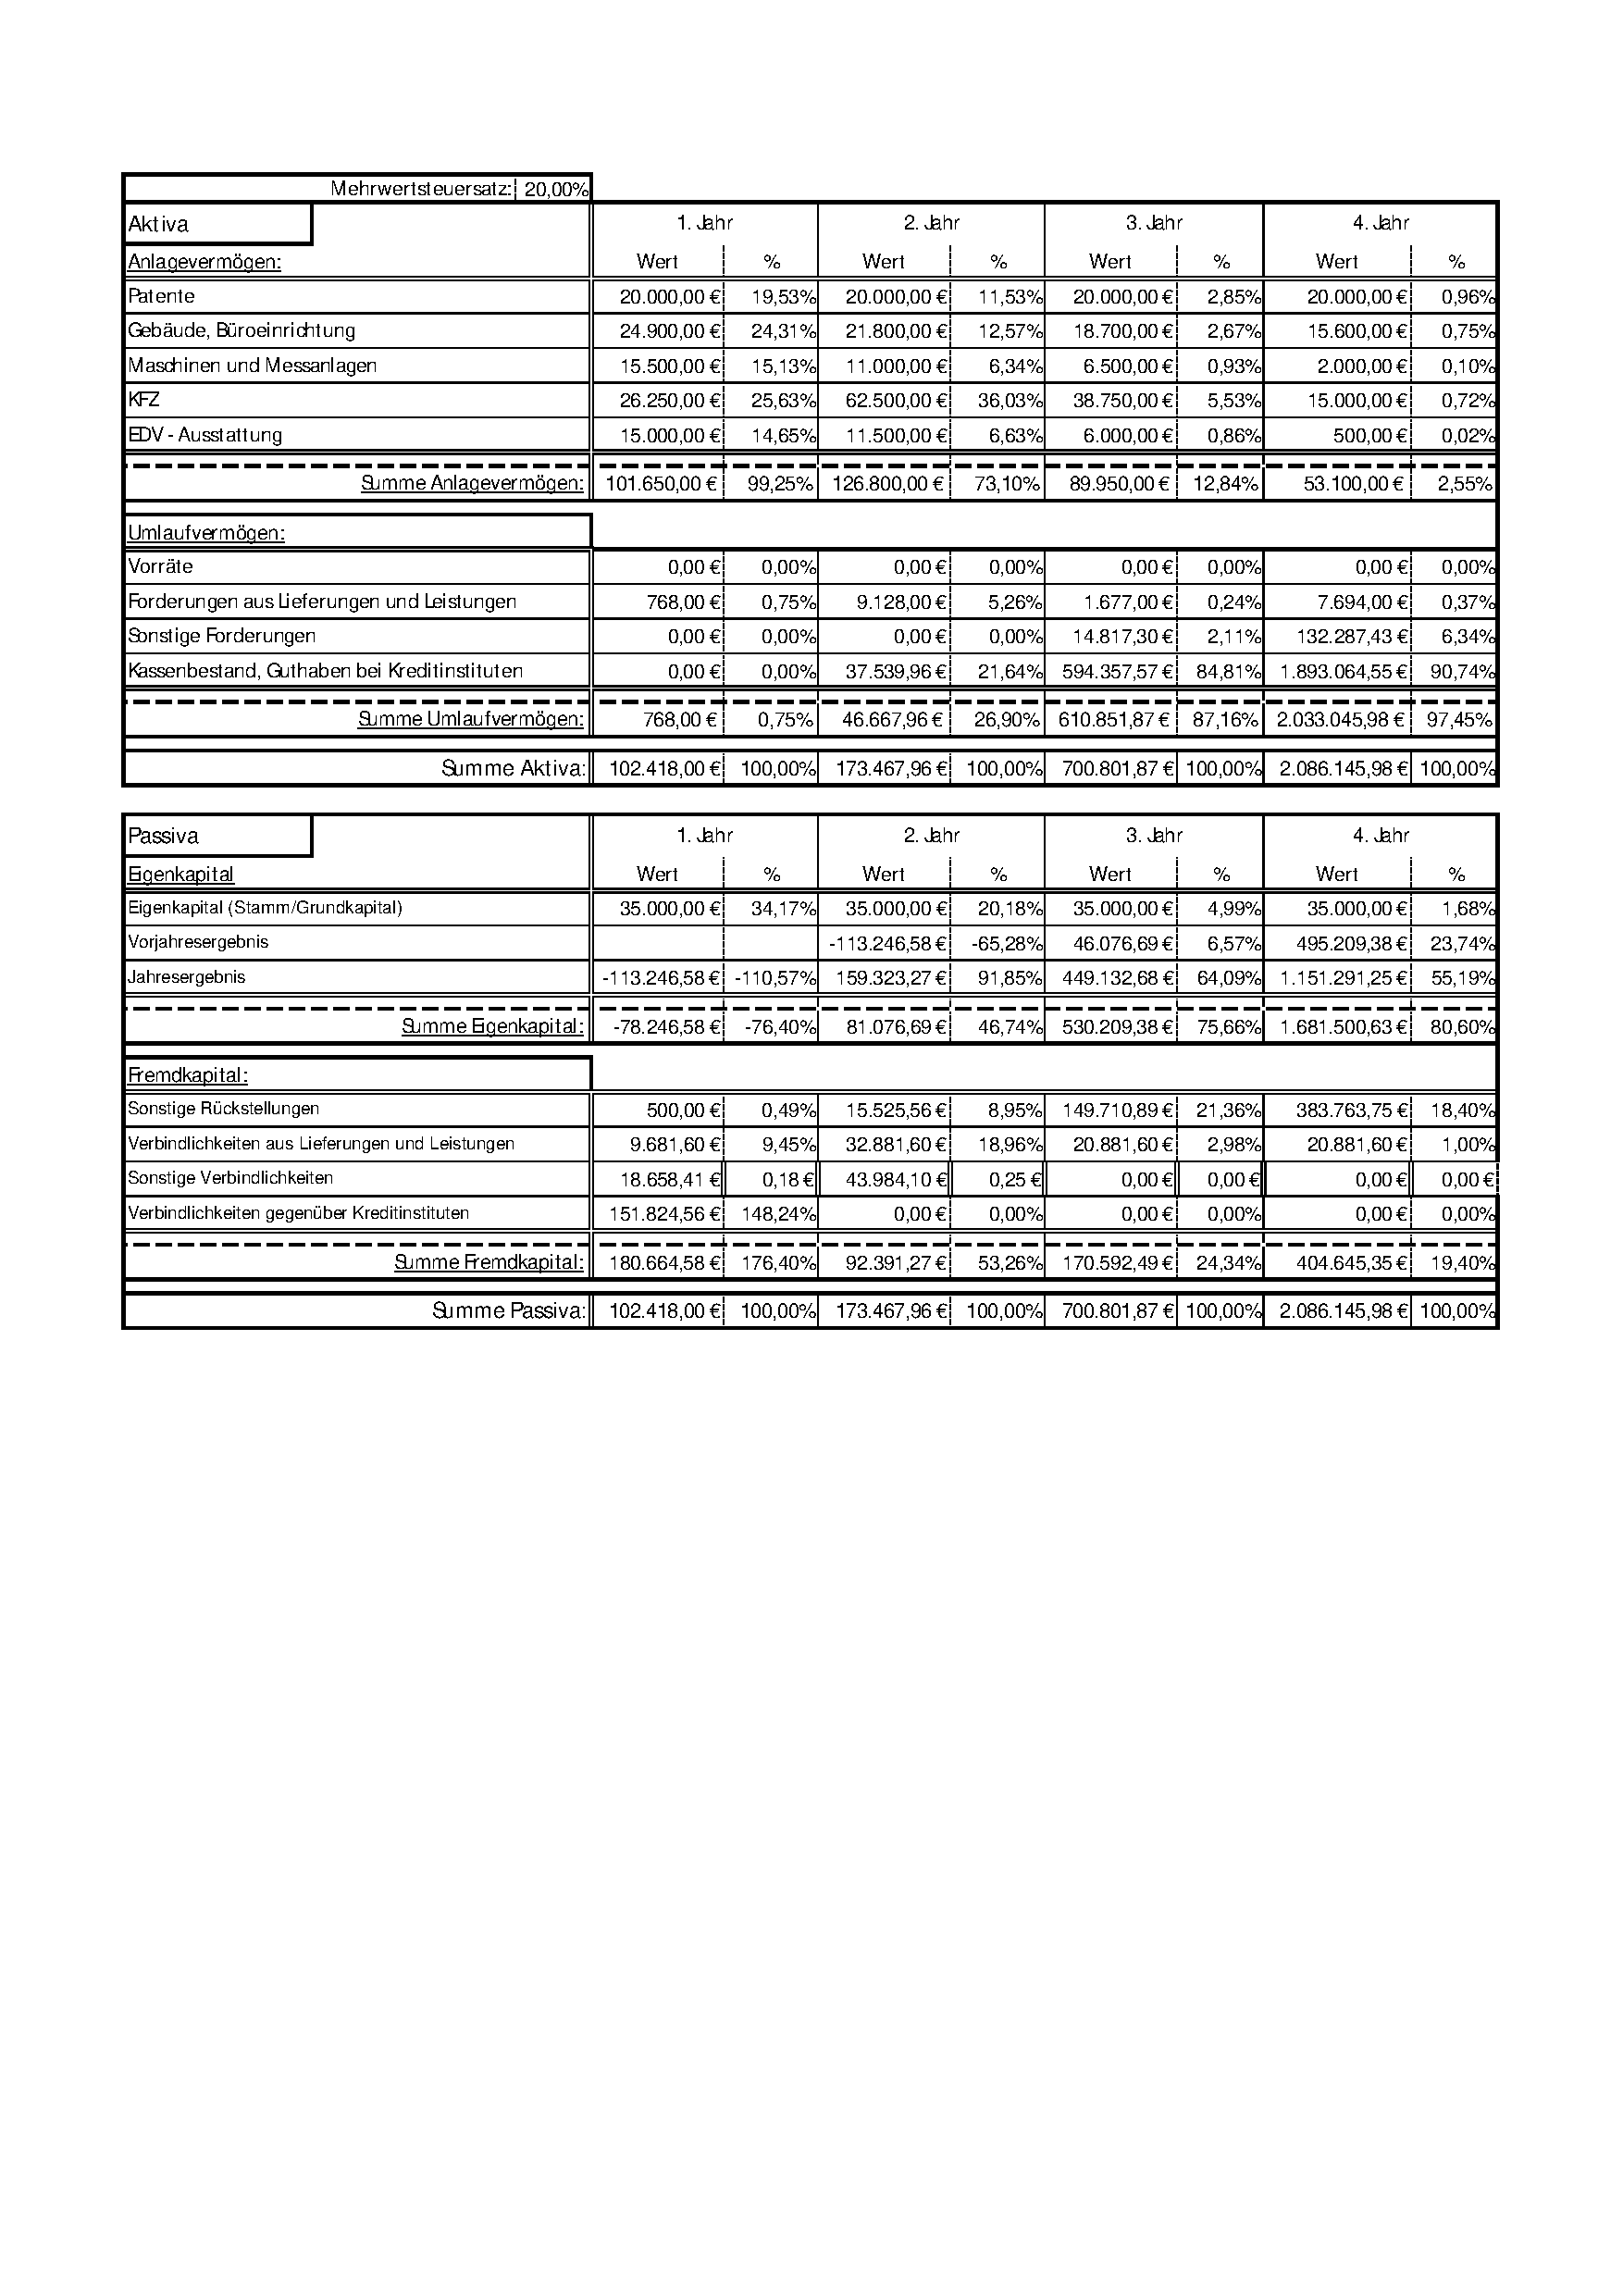
\includegraphics[width=15cm]{BasisSzenario-Planbilanz.pdf}
	\caption{Planbilanz im Basis-Szenario}
	\label{fig:BasisSzenario-Planbilanz}
\end{figure}

\newpage
\subsection{Liquiditätsplan}
\label{sec:BasisSzenario-Liquidität}
\begin{figure}[htp!]
	\centering
	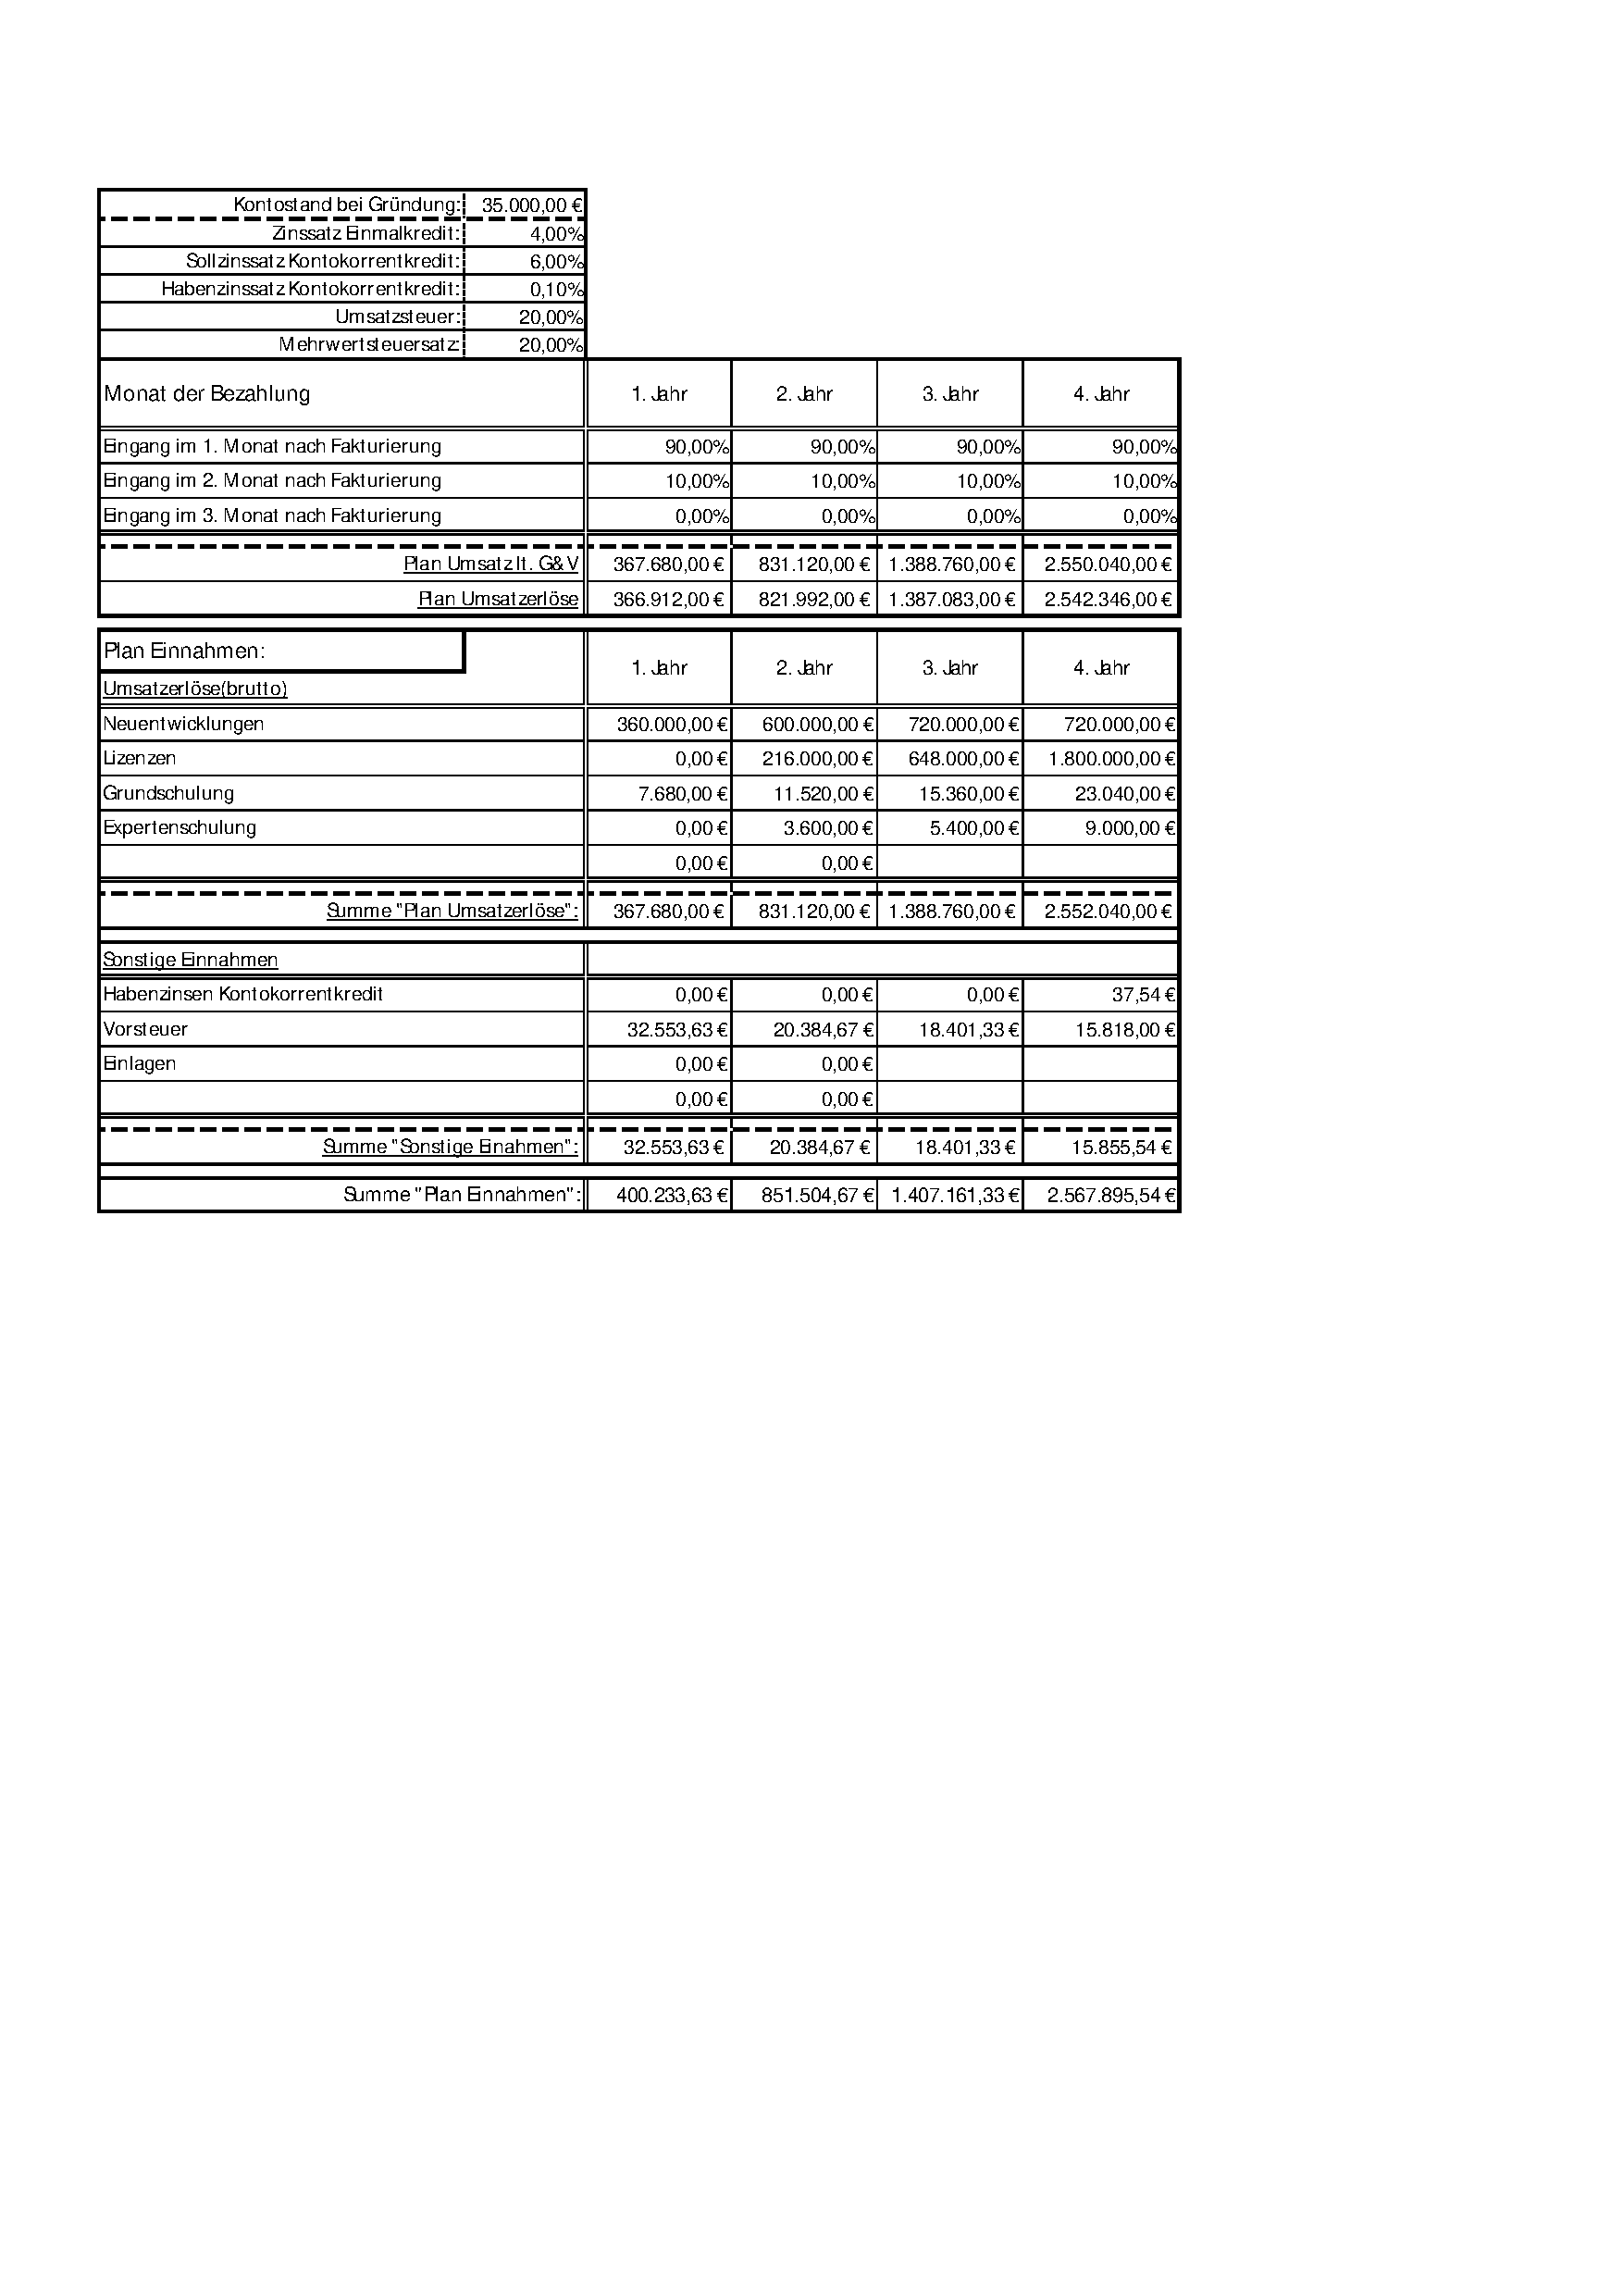
\includegraphics[page=1,width=15cm]{BasisSzenario-Liquiditaet.pdf}
	\label{fig:BasisSzenario-Liquiditaet-1}
\end{figure}
\begin{figure}[htp!]
	\centering
	\includegraphics[page=2,width=15cm]{BasisSzenario-Liquiditaet.pdf}
	\caption{Liquiditätsplan im Basis-Szenario}
	\label{fig:BasisSzenario-Liquiditaet-2}
\end{figure}

\newpage
\subsection{Plan Gewinn- \& Verlustrechnung}
\begin{figure}[htp!]
	\centering
	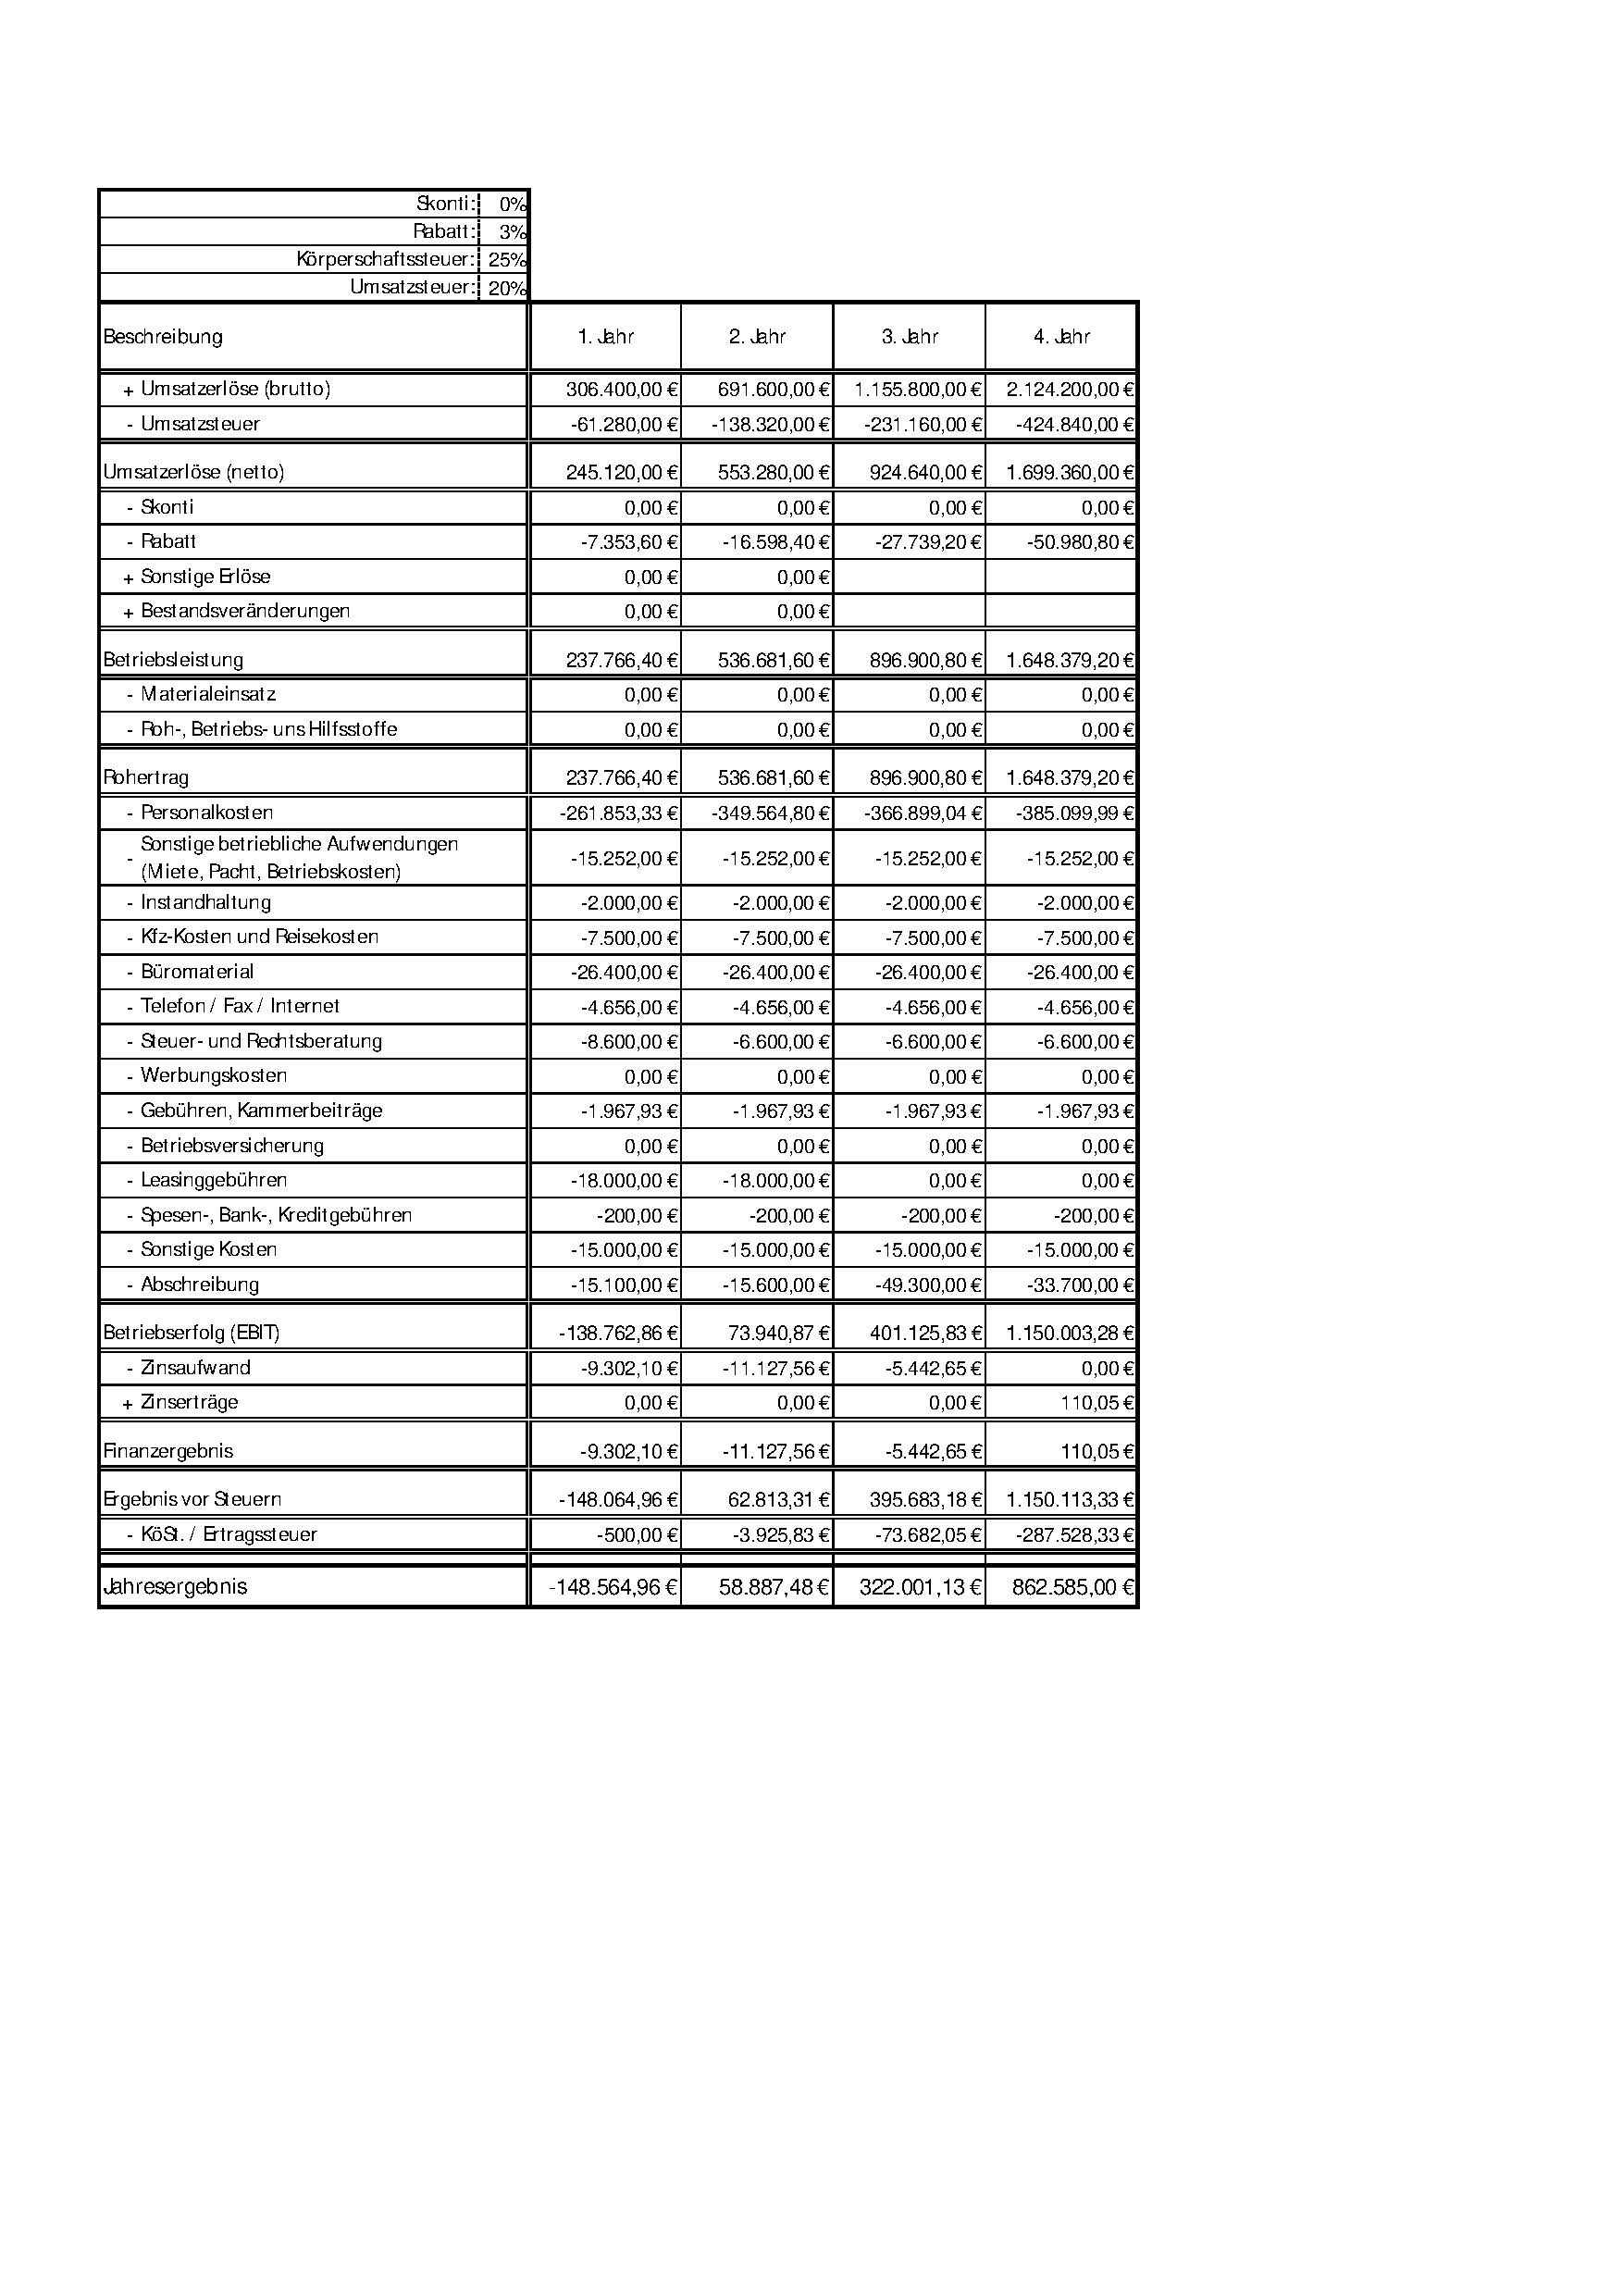
\includegraphics[width=15cm]{BasisSzenario-PlanGuV.pdf}
	\caption{Gewinn- \& Verlustrechnung im Basis-Szenario}
	\label{fig:BasisSzenario-GuV}
\end{figure}

\newpage
\subsection{Investition}
\begin{figure}[htp!]
	\centering
	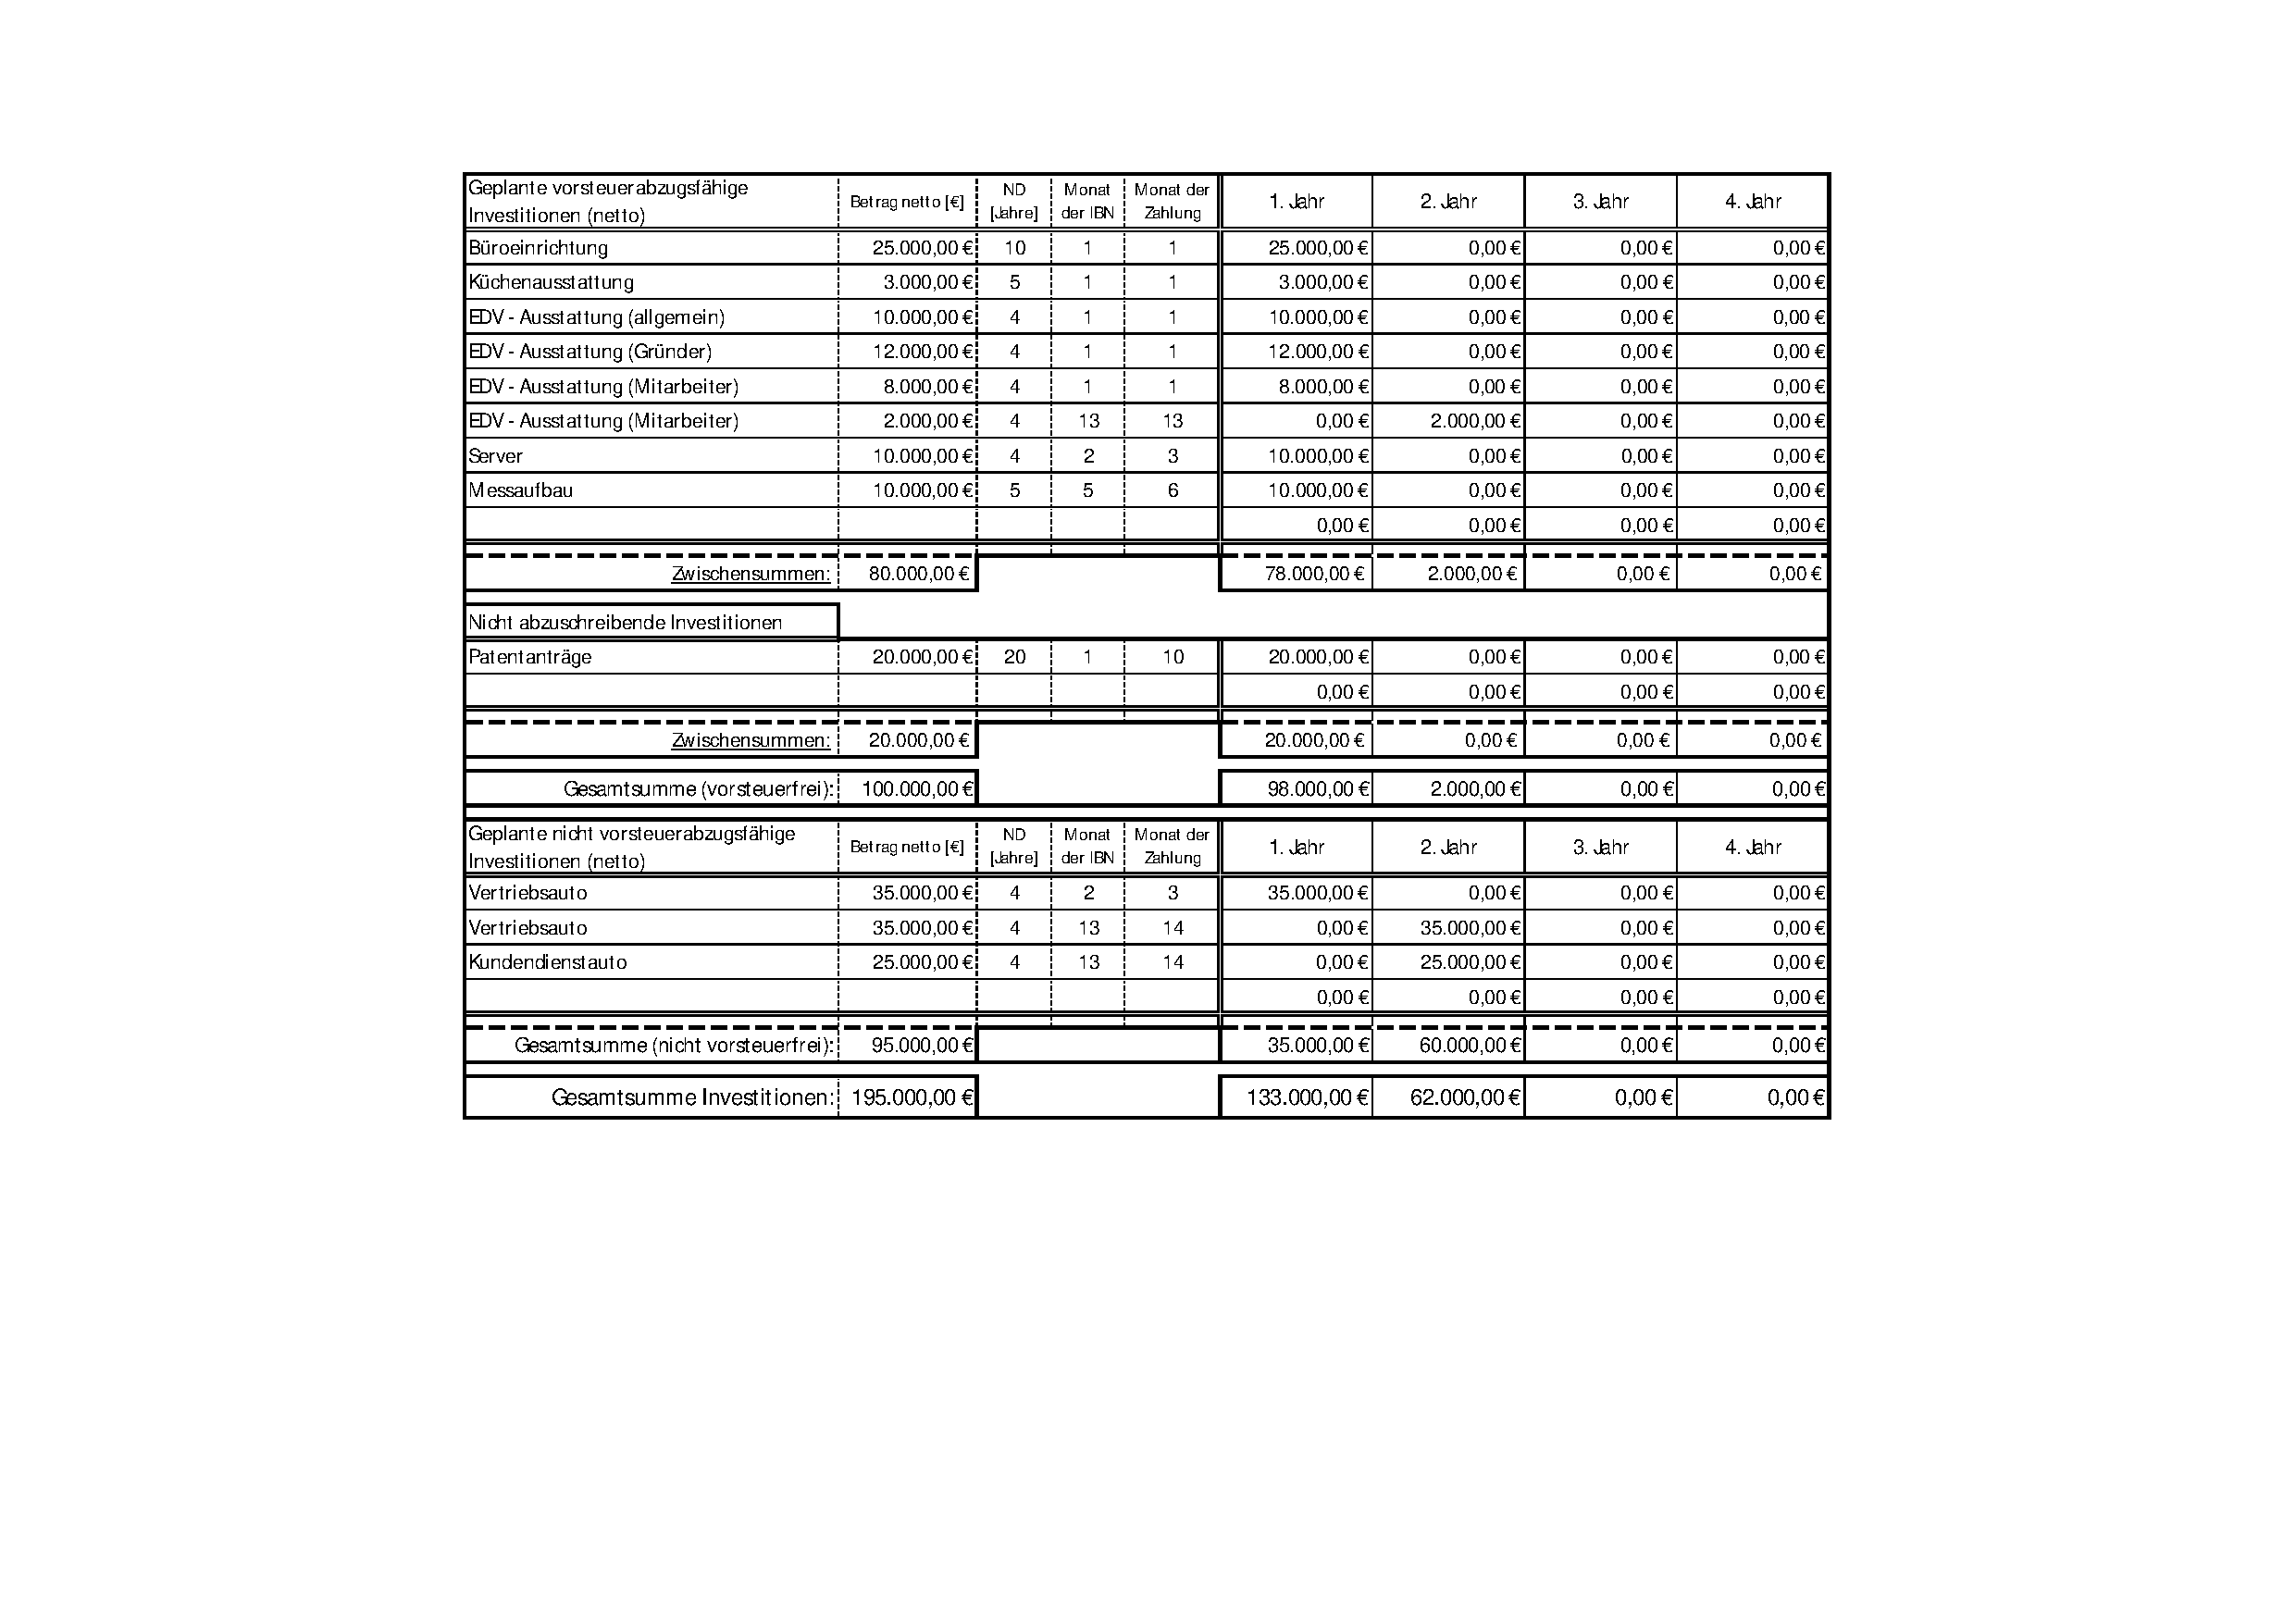
\includegraphics[width=15cm]{BasisSzenario-Investitionen.pdf}
	\caption{Investitionen im Basis-Szenario}
	\label{fig:BasisSzenario-Investitionen}
\end{figure}

\begin{landscape}
	\subsection{Aufwände}
	\begin{figure}[htp!]
		\centering
		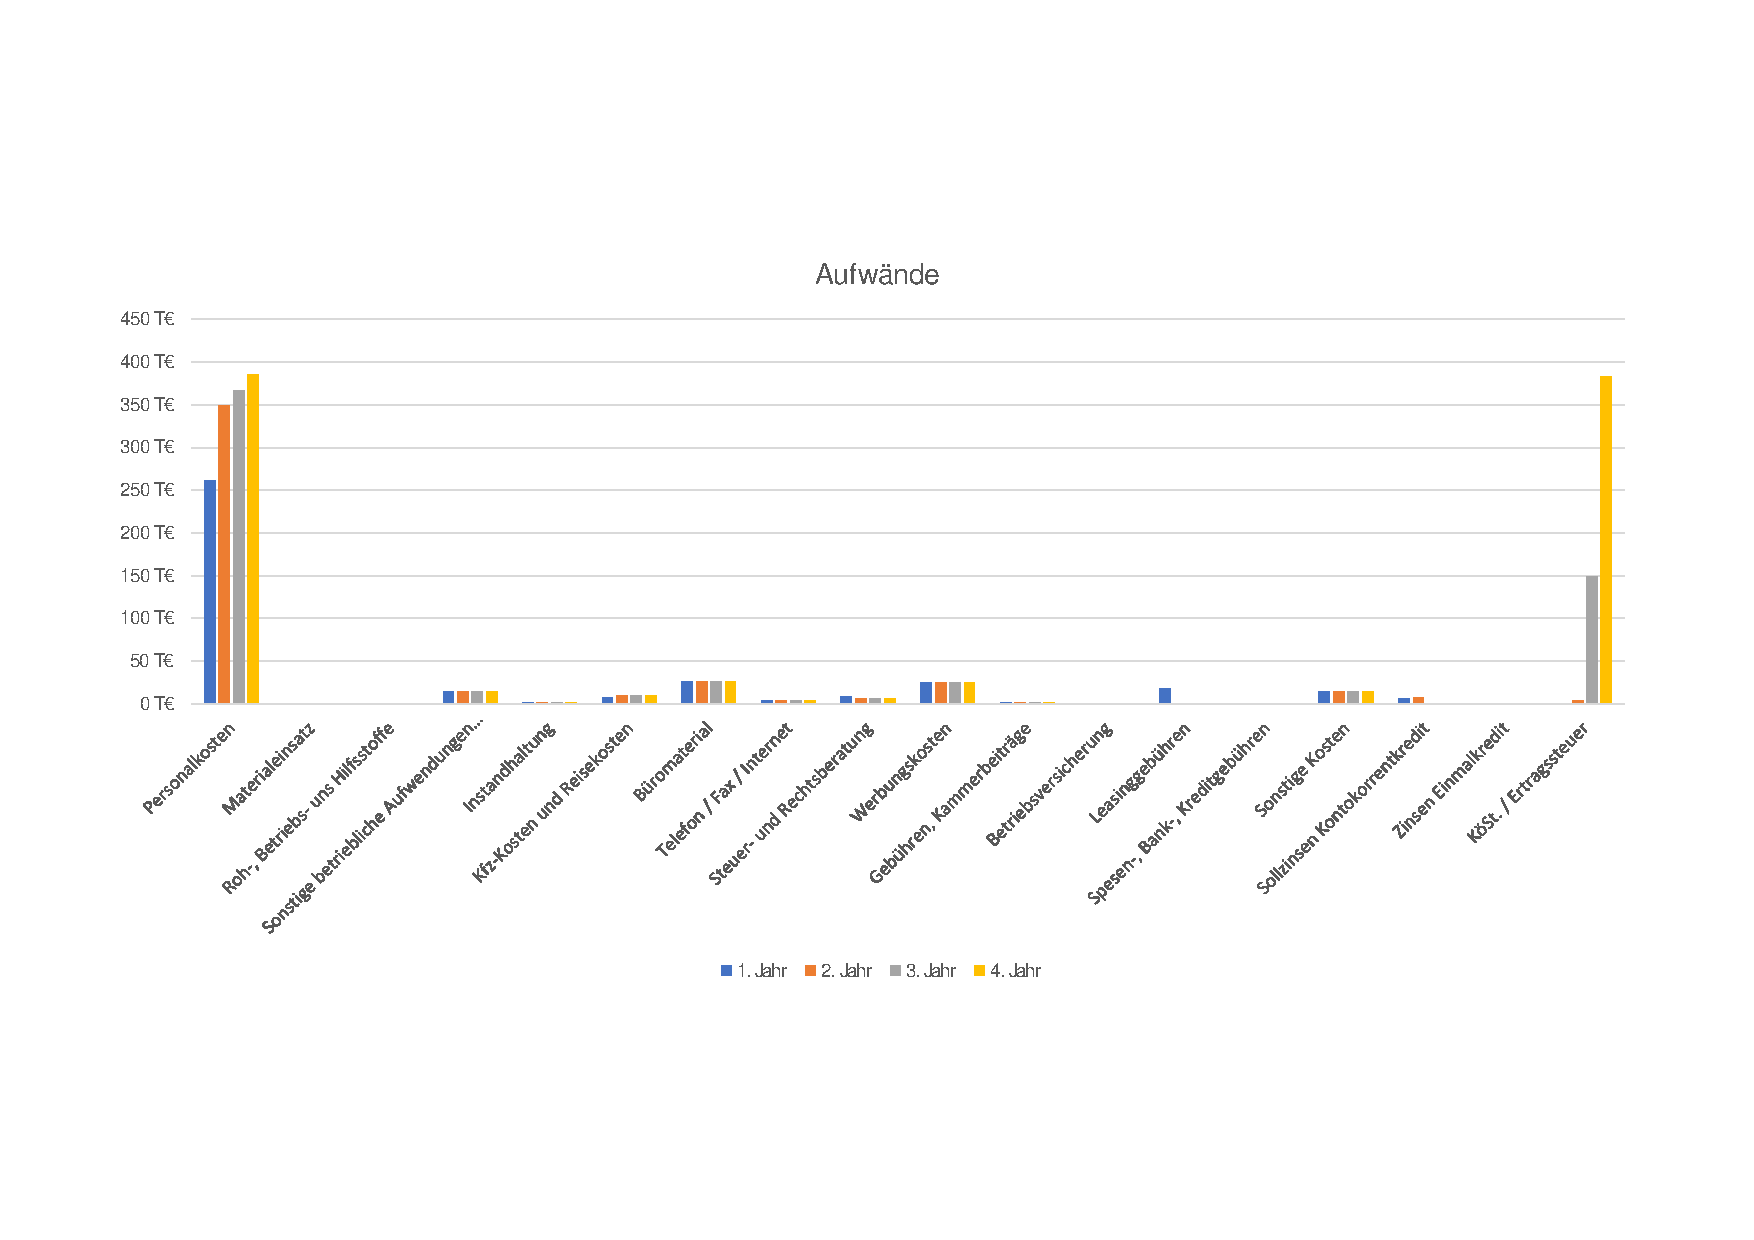
\includegraphics[width=24cm]{BasisSzenario-Aufwaende.pdf}
		\caption{Aufwände im Basis-Szenario}
		\label{fig:BasisSzenario-Aufwaende}
	\end{figure}
\end{landscape}

\subsection{Kapitalbedarf}
Die zurzeit aufgestellt Bilanz wurde unter der Annahme erstellt, dass die Differenz zwischen Kosten und Umsätzen, siehe Kapitel \ref{sec:BasisSzenario-BEP}, über den Kontokorrentkredit (Bankenfinanzierung) gedeckt werden. Grundsätzlich wird die im folgendem Absatz beschriebene alternative Finanzierung angestrebt.

\subsubsection{Alternative Finazierung}
Der Kapitalbedarf bis zum BEP beträgt inklusive einer Reserve und abzüglich der Zinsen des Kontokorrentkredites (siehe Kapitel \ref{sec:BasisSzenario-Liquidität}) höchstens $200.000$ \officialeuro.\\
Um diese Lücke zu schließen, werden folgende Finanzierungsmöglichkeiten geplant:
\begin{itemize}
	\item Einreichung eines Antrags bei der FFG im Basisprogramm zur Förderung von Einzelprojekten.
	\item UBG Gründerfonds
	\item Zusätzliches Eigenkapital
\end{itemize}
Dadurch ergibt sich folgende Finanzierung:\\
\begin{tabular}{l r}
	Kapitalbedarf & $-200.000$ \officialeuro \\
	\hline
	FFG Basisprogramm(Projektsumme: $200.000$ \officialeuro) & $+100.000$ \officialeuro \\
	UBG Gründerfond & $+75.000$ \officialeuro \\
	Fremdkapital der Gesellschafter & $+25.000$ \officialeuro \\
	\bottomrule
\end{tabular}\\

\noindent Im detailliertem Liquiditätsplan ist im ersten Jahr ein Engpass ersichtlich. Dieser erfordert einen zusätzlichen Bedarf von höchstens $55.000,00$ \officialeuro. Dieser kurzfristige Bedarf wird über einen Einmalkredit  einer Bank gedeckt, wobei die vier Gesellschafter von \textsf{RTI GmbH} zu je einem Viertel dafür privat haften.\\
Wird dennoch kein Kredit gewährt, verzichten die vier Geschäftsführer in den ersten sechs Monaten auf ihr Gehalt und die Anschaffung eines Vertriebsautos wird um ein Jahr verzögert.\\

\noindent Kurzfristige Liquiditätsschwankungen (spätere Zahlungen der Kunden, Projektvorfinanzierung, …) werden über einen Kontokorrentkredit gedeckt.

\newpage
\section{Best-Case-Szenario}
Für das Best-Case-Szenario wurden folgende Annahmen getroffen:
\begin{itemize}
	\item Es werden in den folgenden vier Jahren 30 Neuentwicklungen in Auftrag gegeben (Aufteilung:~4/7/9/10). Damit werden $~17,6$\% der Robotertypen der fünf wichtigsten Hersteller mit dem System ausgerüstet, siehe Kapitel \ref{sec:Marketing}.
	\item Die Lizenzvergabe verteilt sich wie folgt:\newline (Angaben in Prozent vom weltweitem Absatz von Industrierobotern ($400.000$ Stück), siehe Kapitel \ref{sec:Marketing})
	\begin{itemize}
		\item 1. Jahr: 0 Roboter
		\item 2. Jahr: 200 Roboter
		\item 3. Jahr: 800 Roboter
		\item 4. Jahr: 4000 Roboter
	\end{itemize}
	\item Die durchschnittliche Lizenzgebühr beträgt $1.500,00$ \officialeuro.\\ Dies entspricht dem Mittelwert für $P_N = 1,50$ kW -- $5,00$ kW und $E_N = 10$\% -- $30$\%.
	\item Es wird mit 120 Teilnehmer an der Grundschulung innerhalb der nächsten vier Jahren gerechnet (Aufteilung:~8/24/36/52). Zusätzlich nehmen 25 Teilnehmer die Expertenschulung in Anspruch (Aufteilung: 0/5/8/12).
\end{itemize}

\subsection{Break-Even-Point}
Der BEP wird im Best-Case-Szenario bereits Anfang des 2. Jahres erreicht, siehe Abbildung \ref{fig:BestSzenario-BEP}.
\begin{figure}[h]
	\centering
	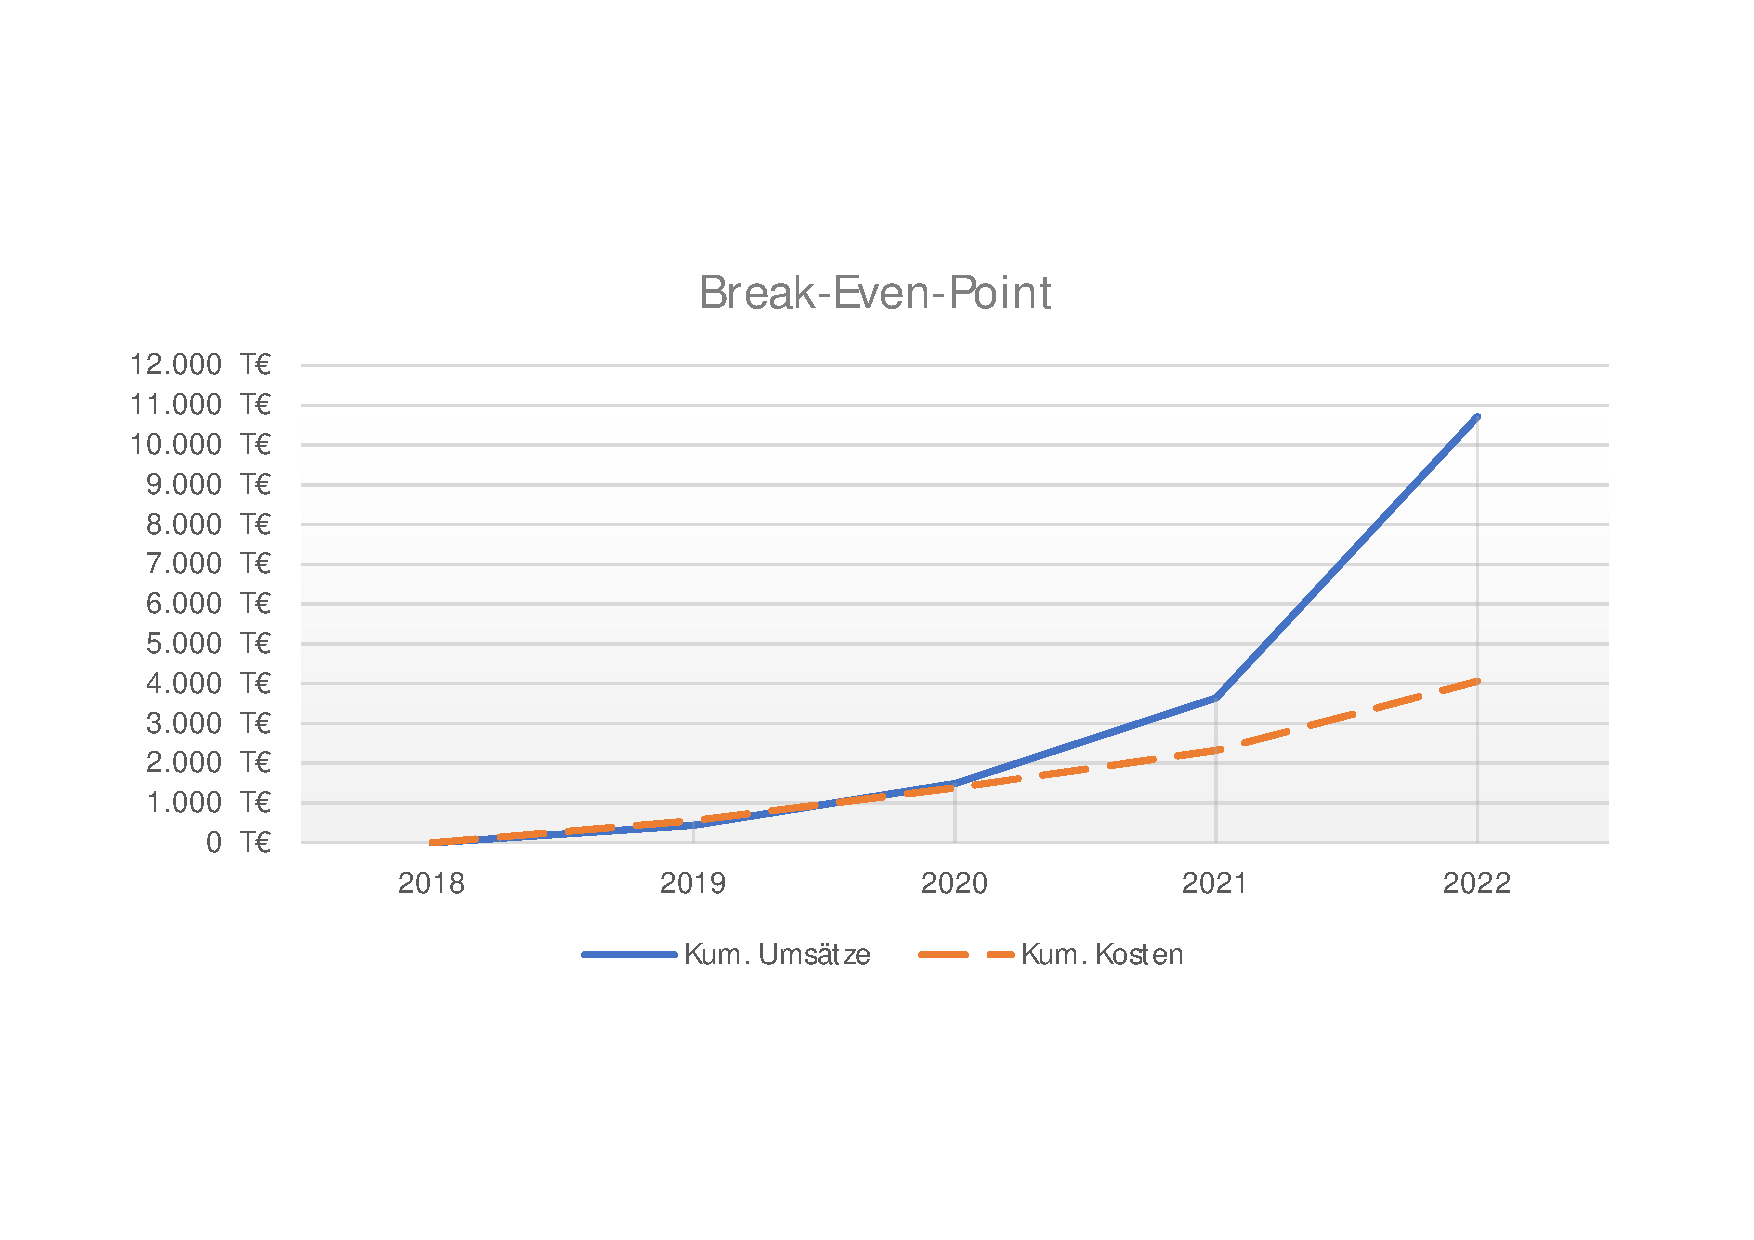
\includegraphics[width=15cm]{BestSzenario-BEP.pdf}
	\caption{Break-Even-Point im Best-Case-Szenario}
	\label{fig:BestSzenario-BEP}
\end{figure}

\subsection{Kapitalbedarf}
Der Kapitalbedarf, inklusive der Berücksichtigung der Liquidität, bis zum BEP beträgt höchstens $175.000$ \officialeuro.\\
Um diese Lücke zu schließen, werden folgende Finanzierungsmöglichkeiten geplant:
\begin{itemize}
	\item Einreichung eines Antrags bei der FFG im Basisprogramm zur Förderung von Einzelprojekten.
	\item UBG Gründerfonds
\end{itemize}
Dadurch ergibt sich folgende Finanzierung:\\
\begin{tabular}{l r}
	Kapitalbedarf & $-175.000$ \officialeuro \\
	\hline
	FFG Basisprogramm(Projektsumme: $200.000$ \officialeuro) & $+100.000$ \officialeuro \\
	UBG Gründerfond & $+70.000$ \officialeuro \\
	\bottomrule
\end{tabular}\\

\noindent Im Gegensatz zum Basis-Szenario wird kein weiterer Einmalkredit benötigt.

\noindent Kurzfristige Liquiditätsschwankungen (spätere Zahlungen der Kunden, Projektvorfinanzierung, …) werden mit einem Kontokorrentkredit abgedeckt.

\newpage
\section{Worst-Case-Szenario}
Für das Worst-Case-Szenario wurden folgende Annahmen getroffen:
\begin{itemize}
	\item Es werden in den folgenden vier Jahren zehn Neuentwicklungen in Auftrag gegeben (Aufteilung:~1/2/3/4). Damit werden $~6$\% der Robotertypen der fünf wichtigsten Hersteller mit dem System ausgerüstet, siehe Kapitel \ref{sec:Marketing}.
	\item Die Lizenzvergabe verteilt sich wie folgt:\newline (Angaben in Prozent vom weltweitem Absatz von Industrierobotern ($400.000$ Stück), siehe Kapitel \ref{sec:Marketing})
	\begin{itemize}
		\item 1. Jahr: 0 Roboter
		\item 2. Jahr: 40 Roboter
		\item 3. Jahr: 120 Roboter
		\item 4. Jahr: 320 Roboter
	\end{itemize}
	\item Die durchschnittliche Lizenzgebühr beträgt $1.500,00$ \officialeuro.\\ Dies entspricht dem Mittelwert für $P_N = 1,50$ kW -- $5,00$ kW und $E_N = 10$\% -- $30$\%.
	\item Es wird mit 25 Teilnehmer an der Grundschulung innerhalb der nächsten vier Jahren gerechnet (Aufteilung:~3/5/7/10). Zusätzlich nehmen sechs Teilnehmer die Expertenschulung in Anspruch (Aufteilung: 0/2/2/2).
\end{itemize}

\subsection{Break-Even-Point}
Der BEP wird im Worst-Case-Szenario erst im 4. Jahr erreicht, siehe Abbildung \ref{fig:WorstSzenario-BEP}.
\begin{figure}[h]
	\centering
	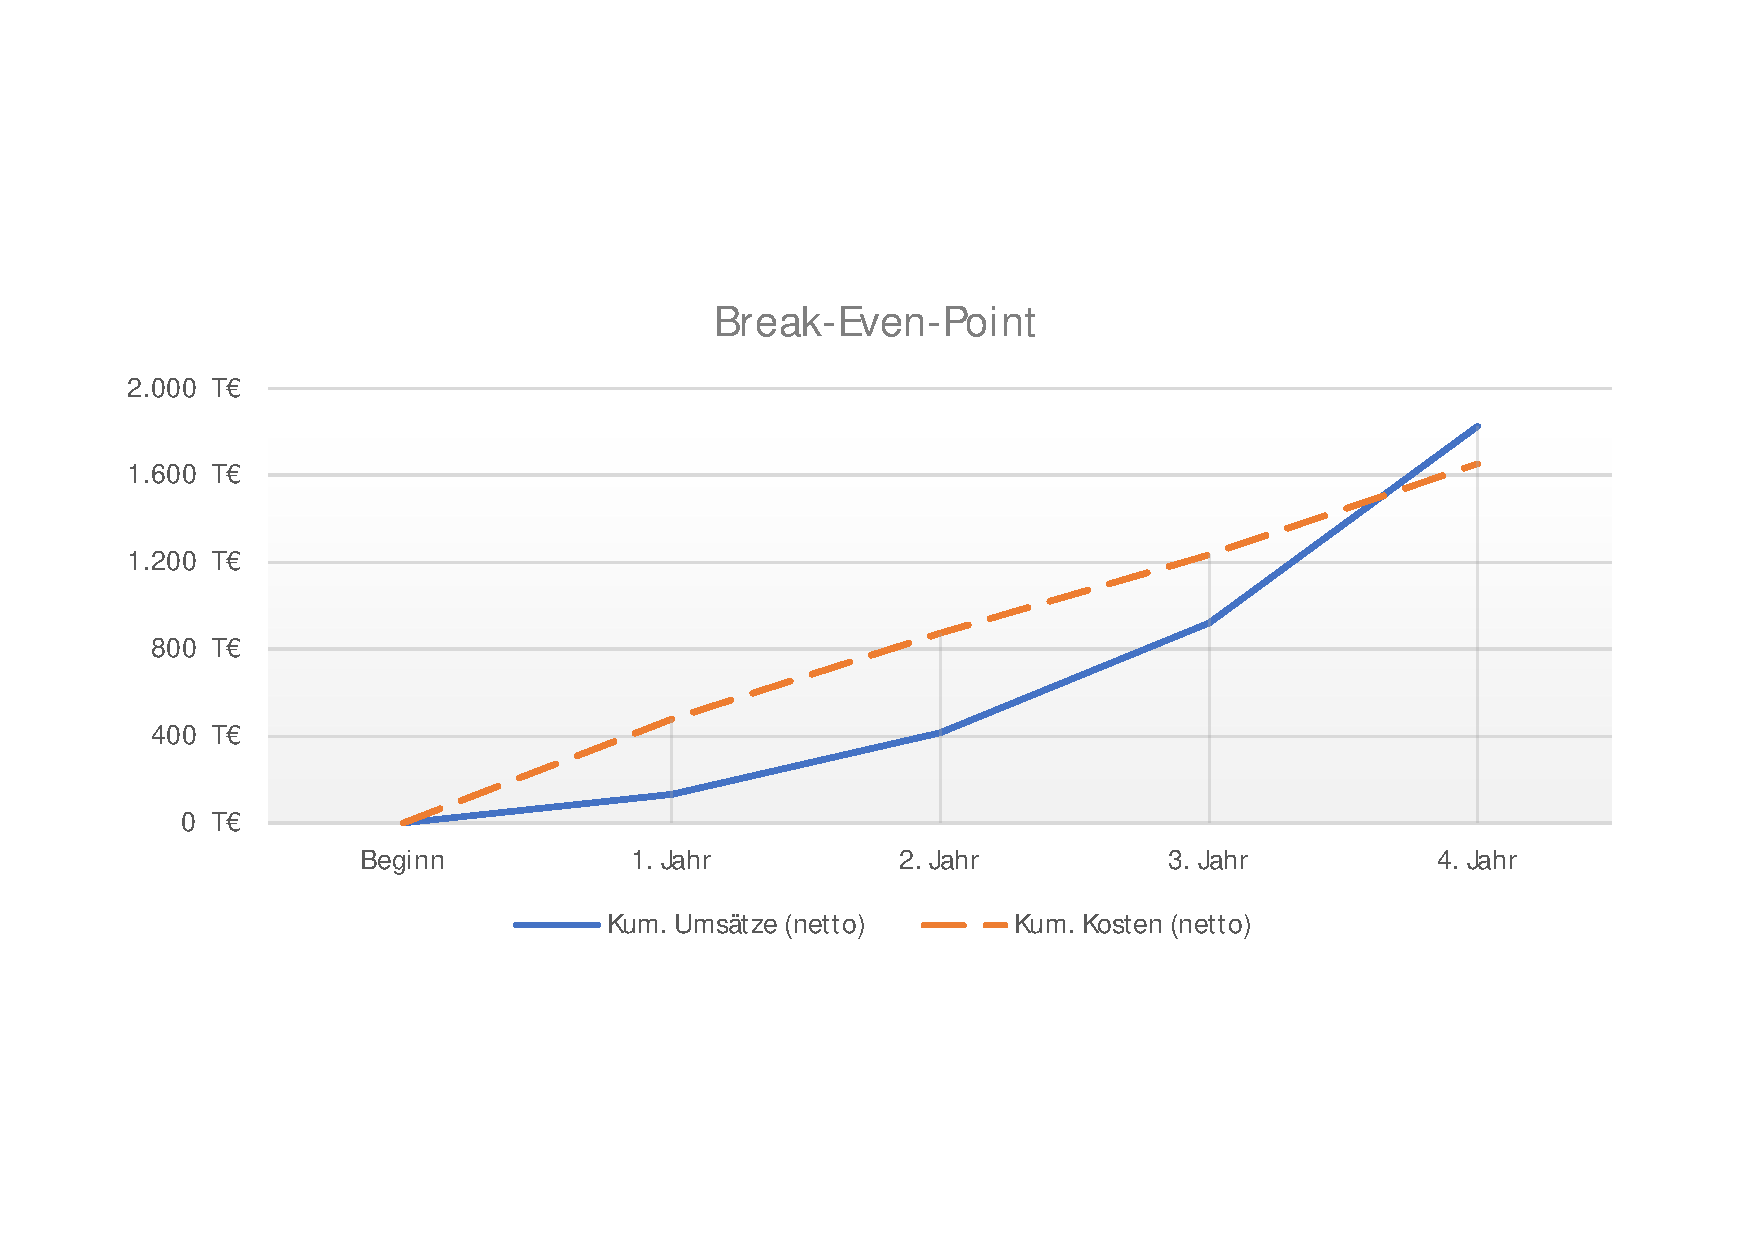
\includegraphics[width=15cm]{WorstSzenario-BEP.pdf}
	\caption{Break-Even-Point im Worst-Case-Szenario}
	\label{fig:WorstSzenario-BEP}
\end{figure}

\subsection{Kapitalbedarf}
Der Kapitalbedarf, inklusive der Berücksichtigung der Liquidität, bis zum BEP beträgt höchstens $435.000$ \officialeuro.\\
Um diese Lücke zu schließen, werden folgende Finanzierungsmöglichkeiten geplant:
\begin{itemize}
	\item Einreichung eines Antrags bei der FFG im Basisprogramm zur Förderung von Einzelprojekten.
	\item UBG Gründerfonds
\end{itemize}
Dadurch ergibt sich folgende Finanzierung:\\
\begin{tabular}{l r}
	Kapitalbedarf & $-435.000$ \officialeuro \\
	\hline
	FFG Basisprogramm(Projektsumme: $200.000$ \officialeuro) & $+100.000$ \officialeuro \\
	UBG Gründerfond & $+75.000$ \officialeuro \\
	\bottomrule
	Differenz: & $-260.000$ \officialeuro
\end{tabular}\\

\textbf{Maßnahmen beim Eintritt des Worst-Case-Szenarios:}
\begin{itemize}
	\item Suche nach strategischen Investoren (Business Angels, Venture Capitalist, Roboterhersteller)
	\item Prüfung alternativer Förderungen
	\item Bankdarlehen im Zuge der FFG-Förderung
\end{itemize}
Kurzfristige Liquiditätsschwankungen (spätere Zahlungen der Kunden, Projektvorfinanzierung, …) werden mit einem Kontokorrentkredit abgedeckt.